
\section{Configuration of the core}
\label{App:PcieCoreConfig}
The Xilinx PCIe core is configured as a PCI express Gen3 (8.0GT/s) core with 8 lanes and the Physical Function (PF0) max payload size is set to 1024 bytes. AXI-ST Frame Straddle is disabled and the client tag is disabled. The reference clock frequency is 100MHz and the only option for the AXI4-Stream interface is 256 bit at 250MHz. Detailed configuration parameters can be seen in Figure~\ref{fig:pcie_core_config1} to \ref{fig:pcie_core_config11}.

\begin{figure}[H]
\centering
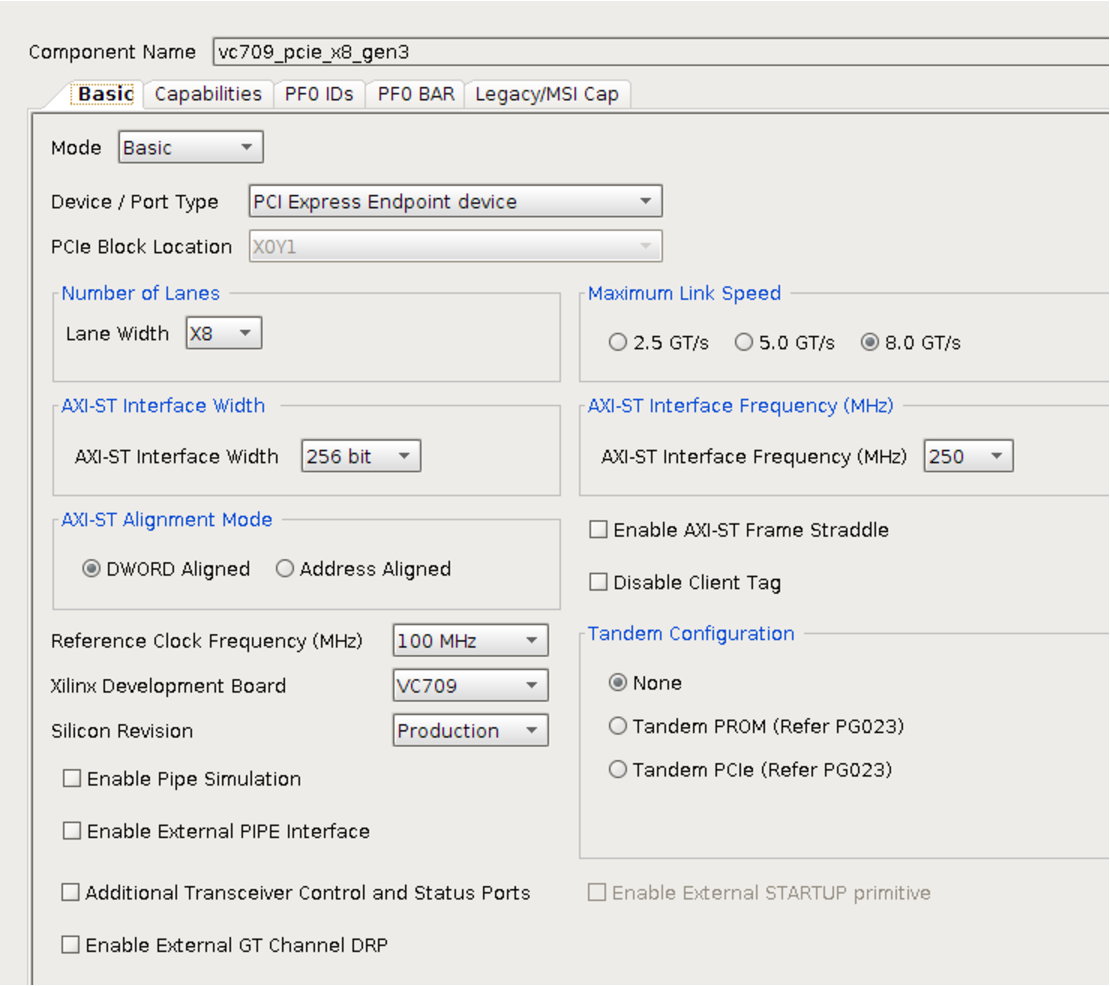
\includegraphics[width=0.75\textwidth]{figures/pcie_core_config1.pdf}
\caption{PCIe core configuration in Vivado [Basic]}
\label{fig:pcie_core_config1}
\end{figure}

\begin{figure}[H]
\centering
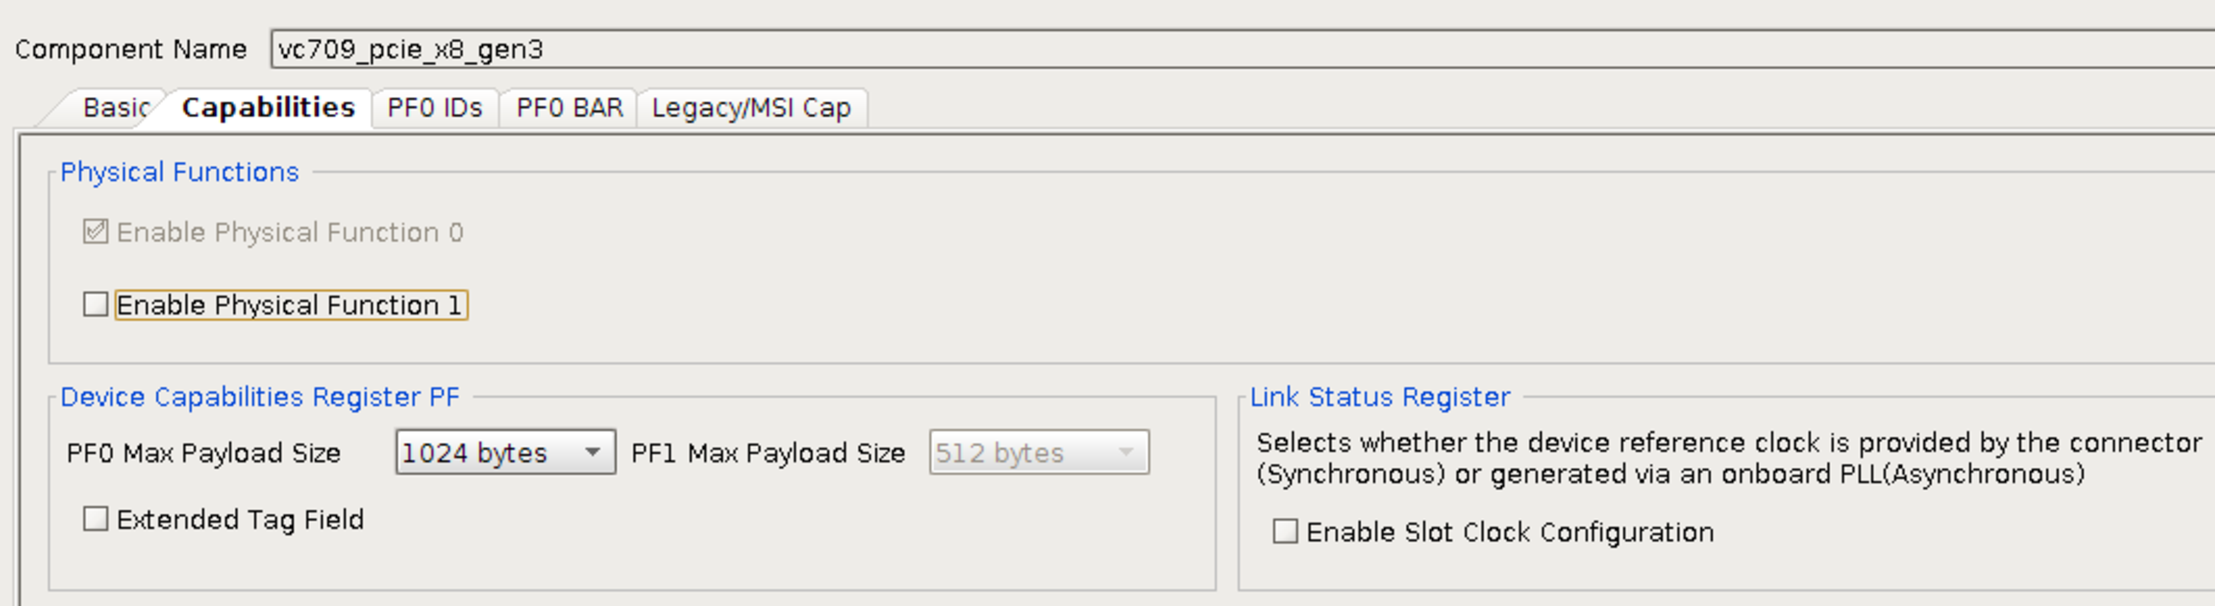
\includegraphics[width=0.75\textwidth]{figures/pcie_core_config2.pdf}
\caption{PCIe core configuration in Vivado [Capabilities]}
\label{fig:pcie_core_config2}
\end{figure}

\begin{figure}[H]
\centering
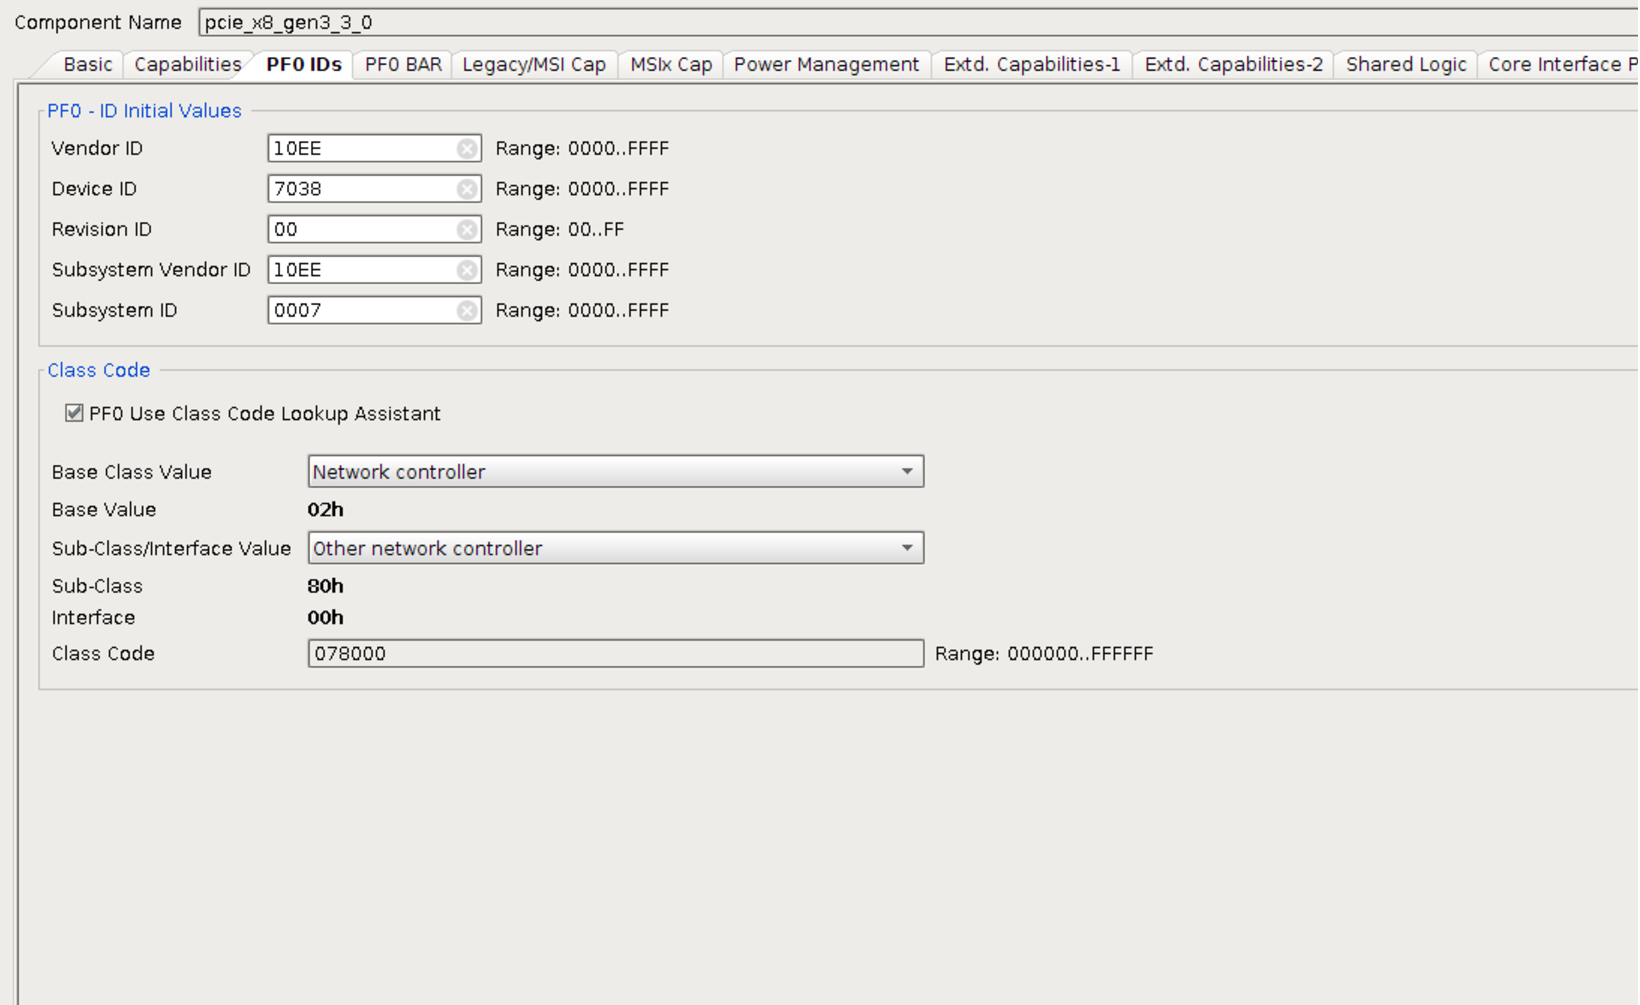
\includegraphics[width=0.75\textwidth]{figures/pcie_core_config3.pdf}
\caption{PCIe core configuration in Vivado [PF0 IDs]}
\label{fig:pcie_core_config3}
\end{figure}
\newpage
\begin{figure}[H]
\centering
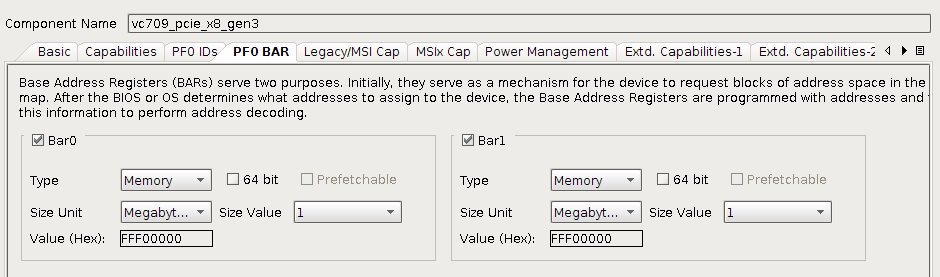
\includegraphics[width=0.75\textwidth]{figures/pcie_core_pf0_bar.png}
\caption{PCIe core configuration in Vivado [PF0 BAR]}
\label{fig:pcie_core_config4}
\end{figure}

\begin{figure}[H]
\centering
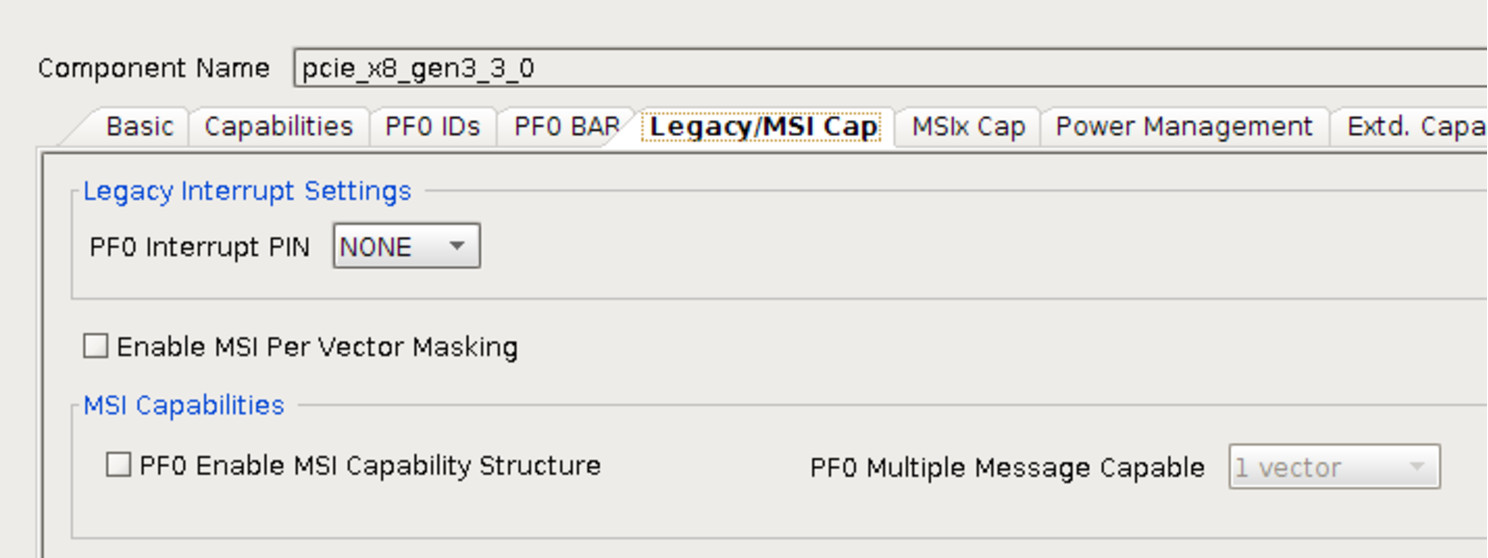
\includegraphics[width=0.75\textwidth]{figures/pcie_core_config5.pdf}
\caption{PCIe core configuration in Vivado [Legacy/MSI Cap]}
\label{fig:pcie_core_config5}
\end{figure}

\begin{figure}[H]
\centering
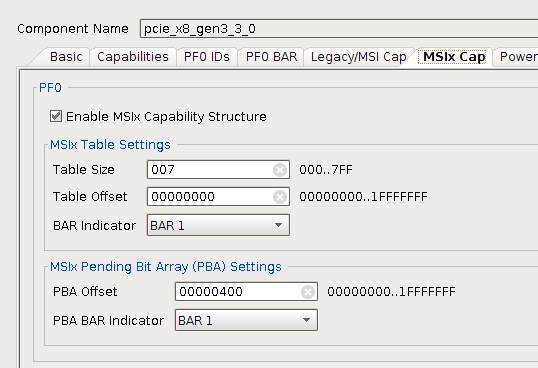
\includegraphics[width=0.75\textwidth]{figures/pcie_core_msix.png}
\caption{PCIe core configuration in Vivado [MSIx]}
\label{fig:pcie_core_config6}
\end{figure}
\newpage

\begin{figure}[H]
\centering
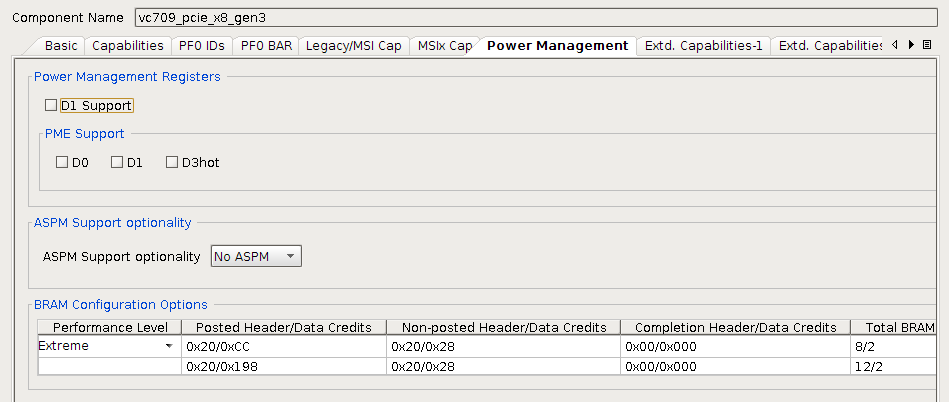
\includegraphics[width=0.75\textwidth]{figures/pcie_core_pwr.png}
\caption{PCIe core configuration in Vivado [Power Management]}
\label{fig:pcie_core_config7}
\end{figure}

\begin{figure}[H]
\centering
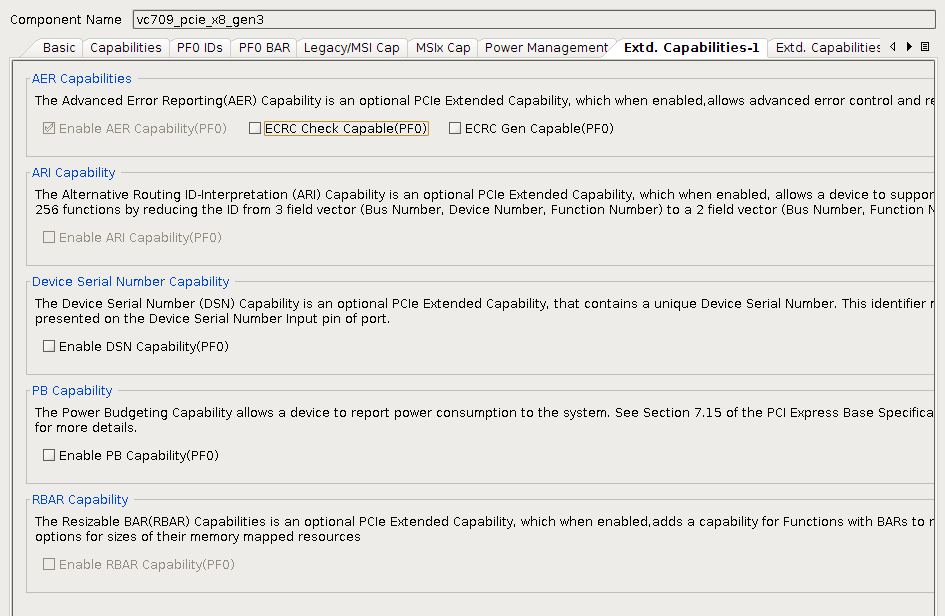
\includegraphics[width=0.75\textwidth]{figures/pcie_core_extcapa1.png}
\caption{PCIe core configuration in Vivado [Extd. Capabilities 1]}
\label{fig:pcie_core_config8}
\end{figure}
\newpage
\begin{figure}[H]
\centering
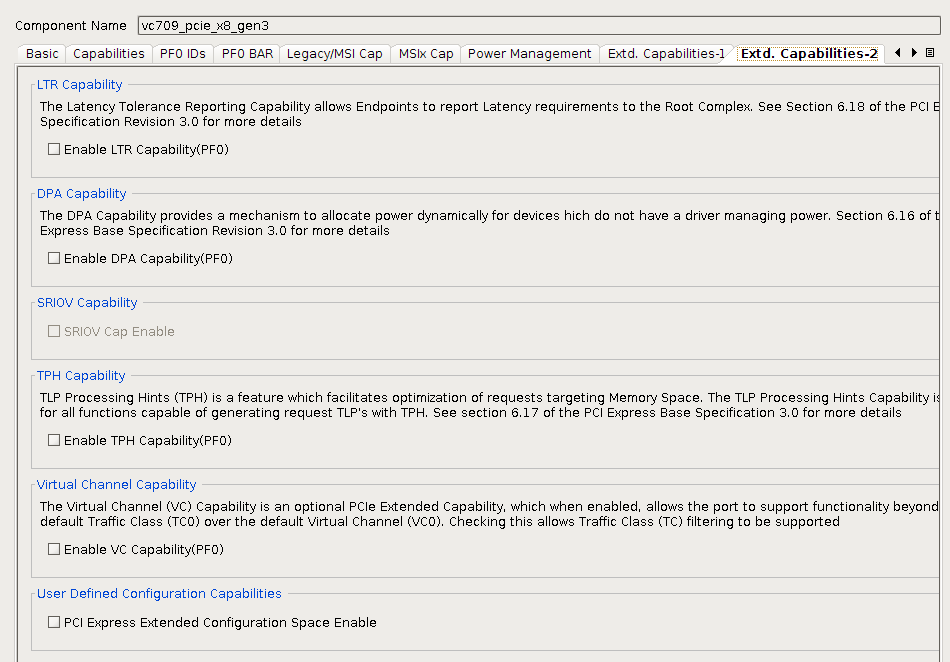
\includegraphics[width=0.75\textwidth]{figures/pcie_core_extcapa2.png}
\caption{PCIe core configuration in Vivado [Extd. Capabilities 2]}
\label{fig:pcie_core_config9}
\end{figure}


\begin{figure}[H]
\centering
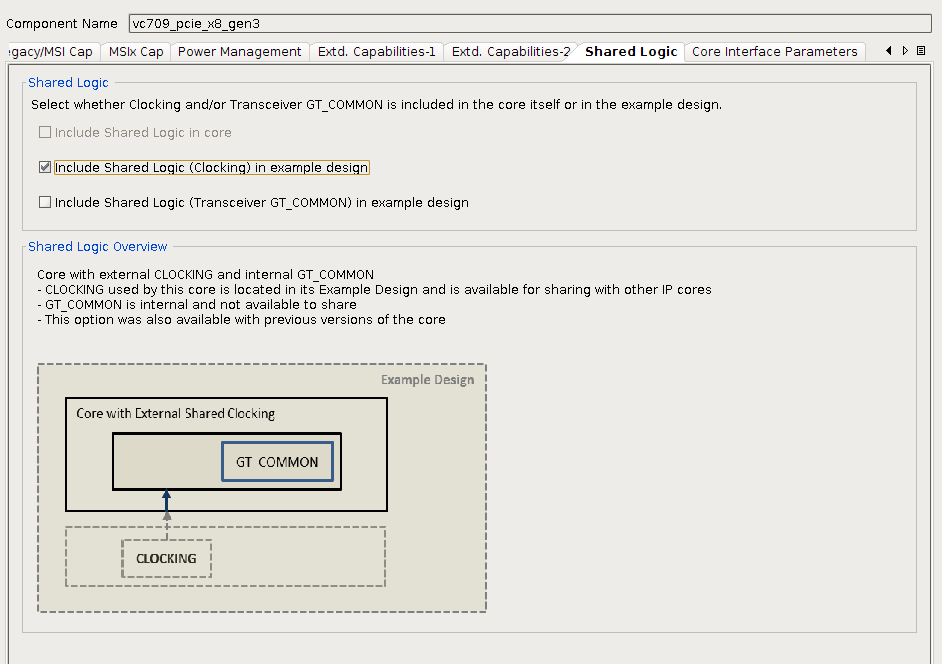
\includegraphics[width=0.75\textwidth]{figures/pcie_core_shared.png}
\caption{PCIe core configuration in Vivado [Shared LogicMSIx]}
\label{fig:pcie_core_config10}
\end{figure}
\newpage
\begin{figure}[H]
\centering
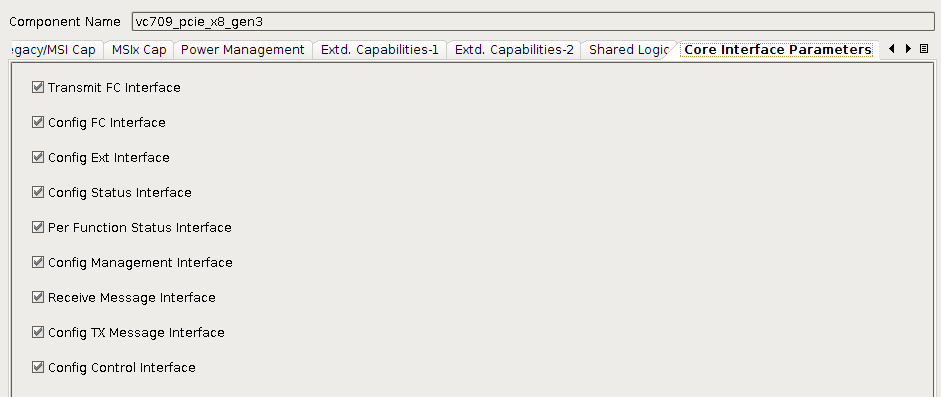
\includegraphics[width=0.75\textwidth]{figures/pcie_core_coreintpar.png}
\caption{PCIe core configuration in Vivado [Core Interface Parameters]}
\label{fig:pcie_core_config11}
\end{figure}
\newpage